\chapter{Development}
\section{Initial testing}
\subsection{Storing questions - Regex}
One of the features that the program requires is an ability to generate random questions. An initial idea was to just store the questions in a text file.
\begin{figure}[H]
	\centering
	\texttt{A ball is projected with speed 20 ms$^{-1}$. At the starting point the ball is 12m of the ground. The highest point of the ball is 20m. Find theta.}
	\caption{Initial question store}
\end{figure} 
The problem with this method is that it is hard to randomise the question. This is because the parts to be randomised in the string are not easily identifiable. 
\begin{figure}[H]
	\centering
	\texttt{A ball is projected with speed [speed]. At the starting point the ball is [height] of the ground. The highest point of the ball is [highpoint]. Find theta.} 
	\caption{Question store with identifiable variables}
\end{figure}
Now the variables can be differentiated from other text, this allows a regular expression to be constructed. The regular expression  will return text enclosed by brackets.
\begin{figure}[H]
	\texttt{import re\\
		question = "A ball is projected with speed [speed]."\\
		variables = re.findall(r'\textbackslash [\textbackslash w+\textbackslash ]', question)\\
		print(variable)\\
		>>> ['[speed]']}
	\caption{Extracting variables from a string using Python regex}
\end{figure} 
This shows how the variables could be extracted using python code. A random number could then be inserted using \texttt{random.randint(range)} function. 

There are downsides to using regular expressions. While it is easy to generalise areas of the string that you would like to capture, the expression can get very complex and hard to maintain. I don't think that I have sufficient experience in using regular expressions to be able to confidently use them in this project, so this method was discarded.
\subsection{Storing questions - String formatting}
Python has built in methods to format strings. This is shown in Figure 2.3 found in Section 2.5.4. This functionality is quite basic, and does not allow you to extract the name of the identifiable variable stored in the string (Figure 3.2). This means that it is hard to extract the name of the variable.

Fortunately there is a way to extend the functionality of the inbuilt Python string formatter, so that it can be customised to your needs. More details about that can be found in PEP 3101\autocite{pep3101}. This shows that you can create a class, that takes a string as an input, and formats the text however you would like it to. 

\begin{figure}[H]
\begin{lstlisting}[language=Python,]
	class object:
	  def __format__(self, format_spec):
	    return format(str(self), format_spec)
\end{lstlisting}
\caption{Example of extended string formatting\autocite{pep3101}}
\end{figure}

This shows how much you can custom the string formatter. An example string for use in this is shown in Figure 2.4.

This method was chosen for use in the project.

\subsection{Graph generation}
There are many Python libraries that allow you to plot graphs and draw diagrams. The most popular library is Matplotlib, which was initially created in 2002 by John Hunter. It allows data to be plotted in a highly customisable way, and interacts very well with Python arrays, which is useful when the data being plotted is generated at runtime.

\begin{figure}[H]
	\centering
	\begin{lstlisting}[language=Python]
	import matplotlib.pyplot as plt
	plt.plot([1,2,3,4])
	plt.ylabel('some numbers')
	plt.show()
	\end{lstlisting}
	
	\caption{Code to create Figure 3.6 \autocite{mpl}}
\end{figure}
This is code used to generate the simple graph seen below.
\begin{figure}[H]
	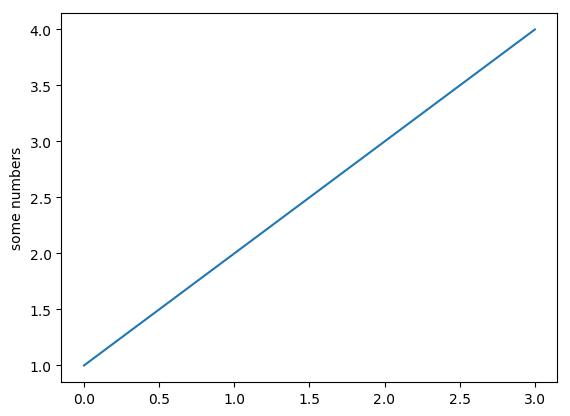
\includegraphics[width=\textwidth,height=\textheight,keepaspectratio]{exmpl.png}
	\caption{Graph generated by code in Figure 3.5}
\end{figure}
The code in Figure 3.5 shows how easy it is to draw a clean looking graph, which would be suitable for use in the program.

Other Python plotting libraries were not looked at, as Matplotlib is perfect for the needs of the project. It is also part of the Anaconda platform\autocite{conda} which is a Python installation containing many scientific Python libraries.  This library was chosen for use in the project.

\subsection{GUI}
There are hundreds of libraries to display GUI's in Python, but there are three that are most commonly used which are:
\begin{itemize}
	\item Tkinter
	\item PyQT
	\item WxPython
\end{itemize}
These are all Python wrappers for C/C++ code, which can make development hard because in some cases error codes may not be returned to the Python console, so you don't know what you have done wrong.

WxPython was immediately discounted, as it does not have stable support for Python version 3.x .

Next tkinter was considered. tkinter is a Python wrapper of Tcl/tk. It is class based, so to create a GUI you must create a class that extends the base frame class, and to customise this frame, you must override methods from the parent class. While the code is not that complex itself, the positioning of elements can get very complex, as it must be done entirely in code, as there is no WYSIWYG\footnote{What you see is what you get.} editor. As this project has a time constraint, tkinter was discarded.

Lastly PyQt was looked at. PyQt is a Python wrapper for Qt, which is a highly popular GUI framework, which is even used for the main touchscreen in the Tesla Model S. Qt comes with an excellent WYSIWYG editor, allowing you to easily create a GUI without having to worry about the code behind it. The code generated however is in C, which would be hard to integrate with the other Python code.

Luckily, there is a program called PyUIC5, which converts C code used to display a Qt GUI, into Python code that performs exactly the same function. This is the perfect tool for this project, as it allows the GUI to be created easily, and functionality to be easily added to the buttons, by extending some classes in the Python code.

Here is how the GUI design workflow will work with PyQt:
\begin{enumerate}
	\item Design GUI in QtCreator
	\item Convert generated C code into Python
	\item Add functionality to buttons in Python code
\end{enumerate}

PyQt was chosen as the GUI tool.

\subsection{Summary}
\begin{itemize}
	\item Extending the Python string formatter for storing questions
	\item Matplotlib for drawing the graphs
	\item PyQt for displaying the GUI
\end{itemize}
\section{Storing questions}
I decided to program each element of the program separately first, and then to integrate them all at the end.
